%======================================================================
%   Zak Webb
%   Ph. D. Thesis
%   Department of Physics and Astronomy
%   University of Waterloo
% 
%   Universality of single-particle scattering
%======================================================================


\documentclass[../thesis-main/thesis-main]{subfiles}
\begin{document}

\chapter{Universality of single-particle scattering}
\label{chap:SP_universality}

%%%%%%%%%%%%%%%%%%%%%%%%%%%%%%%%%%%%%%%%%%%%%%%%%%%%%%%%%%%%%%%%%

With the basic understanding of scattering on graphs, we should be able to combine several graphs so as to show that single-particle quantum walks are universal.  While this has already been shown by Andrew Childs \cite{Chi09}, this is a slightly different graph and analysis, which will help with the understanding of the multi-particle case.  In particular, the method for encoding a computation will be to have a long (but finite) path for each computational basis state of the circuit.  We will use several graphs from the previous section so that each gate is implemented with a scattering event.  

While the overall graph will be exponential in size, each individual scattering event will only involve either two or four semi-infinite paths, as our choice of universal gate set only mixes at most two computational basis states per gate.  As such, we will be able to analyze the evolution of a sufficiently large wavepacket, and show that the evolution of such a wavepacket follows the expected evolution for a single gate.  By then combining the graphs in such a manner, we will then be able to show that the final location of the wavepacket can be used to evaluate whether the simulated circuit accepts.


%%%%%%%%%%%%%%%%%%%%%%%%%%%%%%%%%%%%%%%%%%%%%%%%%%%%%%%%%%%%%%%%%

\section{Single-gate blocks}
\label{sec:single_gate_blocks}

Before we encode an entire computation into the evolution of a quantum walker, we first need to be able to encode a single gate.  To do this, we will use the results of \chap{scattering_on_graphs}, as we have already shown how to simulate the evolution of a universal gate set.  Unfortunately, the results of that section do require that each of the input and output paths to be semi-infinite, which will be problematic for combining these evolutions in series.

However, if we examine \lem{SP_wavepacket}, we can see that for all times of interest, most of the amplitude remains close to the graph.  Intuitively, we would thus expect the evolution for these times to remain mostly unchanged if we then remove those vertices far from the graph.  This is actually the bulk of the \lem{NPL}, which we will use to great effect in our proof.

Before we analyze the actual evolution, however, we will want to construct these small graphs themselves.  As such, let us assume that we are working with $n$ qubits, and let us assume that we are applying the unitary $U$, where $U\in \{H, T,\CNOT\}$.  With this assumption, the graph corresponding to  a single gate will then consist of $2^{n+1}$ paths of length $2M+L$, where $M$ and $L$ are integers to be determined, along with a scattering graph $G_U$ that implements the appropriate unitary evolution.  Half of the long paths will correspond to the input paths, while the other half will correspond to the output paths.  We will then connect these paths to the input and output vertices of $G_U$.   In particular, the graph will look like \fig{SP_block}.  

\todo{fix figure}

\begin{figure}
  \centering
  \tikzsetnextfilename{SP_block}
  %%%%%%%%%%%%%%%%%%%
%  This is the TikZ code for the single-particle block idea.  In particular, this contains code for stuff.
%

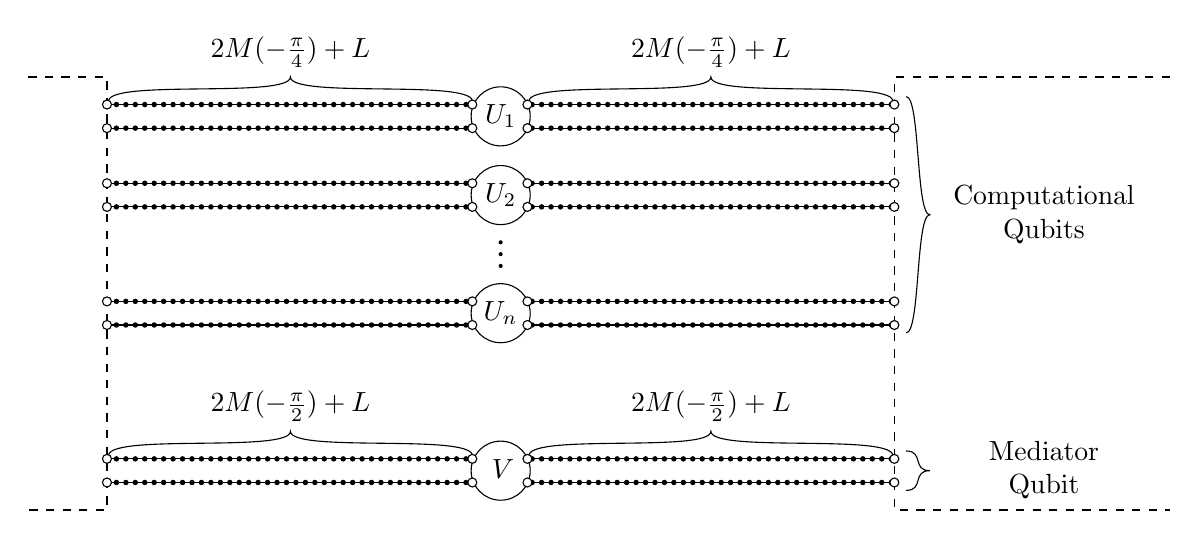
\begin{tikzpicture}[
  unitary/.style={circle,draw=black,fill=white,
    inner sep=0pt,minimum size=7.5mm},
  dots/.style={circle,fill=black,
    inner sep=0pt,minimum size=1.5pt},
  vert/.style={circle,fill=black,
    inner sep=.7pt,minimum size=0pt},
  attach/.style={circle,draw=black,fill=white,inner sep=1.15pt,minimum size=0}]

  \foreach \n /\y in {U_1/2.5,U_2/1.5,U_n/0,{V_{\med}}/-2}{
    \begin{scope}[yshift = \y cm]
      \foreach \x in {0,.12,...,10} {
        \node at (\x, -.15) [vert] {};
        \node at (\x, .15) [vert] {};
      }
      \draw (0, -.15) to (10, -.15);
      \draw (0,  .15) to (10,  .15);
      \node at (5,0) [unitary]{$ \n $};


    \end{scope}
  }
  
  \foreach \x in {0,5.34}{
  \foreach \y /\p in {2.5/4,-2/2}{
  \begin{scope}[xshift=\x cm,yshift=\y cm]
    \node (\x\p) at (2.33,.5)[above] {$2M(-\frac{\pi}{\p}) + L$};
  
    \draw (0.02,0.2) to[out=80,in=-90,looseness=0.3] (2.33,.5)
                     to[out=-90,in=100,looseness=0.3] (4.64,.2);
  \end{scope}}} 
                  
  \draw (10.15,2.75) to[out=0,in=-180,looseness=0.3] (10.45,1.25)
                    to[out=-180,in=0,looseness=0.3] (10.15,-.25);
  \node at (11.9,1.25)
      {\begin{tabular}{c}
          Computational\\ 
          Qubits\end{tabular}};


  \draw (-1,3) to (0, 3) to (0,-2.5) to (-1,-2.5) [dashed];
  \draw (13.5,3) to (10,3) to (10,-2.5) to (13.5,-2.5) [dashed];

  \node at (5,.9) [dots] {};
  \node at (5,.75)    [dots] {};
  \node at (5,.6) [dots] {};

  \draw (10.15,-1.75) to[out=0,in=-180,looseness=1.5] (10.45,-2)
                    to[out=-180,in=0,looseness=1.5] (10.15,-2.25);
  \node at (11.9,-2) 
      {\begin{tabular}{c}
          Mediator\\ 
          Qubit\end{tabular}};
          
   \foreach \x in {0, 10, 4.64, 5.34}{
   \foreach \y in {2.35,2.65,1.65,1.35,.15,-.15,-1.85,-2.15}{
     \node at (\x, \y) [attach] {};
   }}
\end{tikzpicture}
  \caption{The intuitive idea for a single-particle block.}
  \label{fig:SP_block}
\end{figure}

Additionally, as the scattering behavior of graphs is intrinsically related to the momentum of the wavepackets, we will need to decide on this before we finish the construction.  In anticipation of \chap{MP_universality}, as well as the simplicity of certain graphs, our construction will utilize $k = -\dfrac{\pi}{4}$.

%%%%%%%%%%%%%%%%
\subsection{Construction of $G_U$}

With these choices, the graphs for $G_U$ will be relatively simple.  For all graphs except for the amplitude mixing gate, the subgraphs will simply consist of paths, so that the evolution will essentially just be the same as on a long path, possibly with an encoded change of phase.  For the amplitude mixing gate, things will be slightly di

If $U$ is a $\Tgate$-gate acting on qubit $j$, then the graph $G_U$ will consist of $2^{n-1}$ paths of length $2$ connecting input $x_{\text{in}}$ to $x_{\text{out}}$, where $x_j = 0$, and $2^{n-1}$ paths of length $1$ connecting input $x_{\text{in}}$ to output $x_{\text{out}}$ where $x_{j} = 1$.  In this manner, the scattering amplitude will always have perfect transmision, and different momenta will only result in a different encoded gate (namely that this will be a $-\dfrac{k}{2}$-phase gate as opposed to a $\dfrac{\pi}{8}$-gate.

If $U$ is a $\CNOT$-gate controlled by qubit $i$ and acting on qubit $j$, then this is even more simple than the $\Tgate$-gate.  In particular, the graph $G_U$ will consist of $2^n$ paths of length 2, where input $x$ is connected to output $y$, where $x_k = y_k$ for all $k\neq j$, and $y_j =x_i + x_j - 2 x_i x_j$. 

Finally, if $U$ is the Basis-changing gate acting on qubit $j$, then things become slightly more complicated.  In particular, $G_U$ then consists of $2^{n-1}$ copies of the graph \fig{basis_change}, with inputs $x_{\text{input}}$ and $y_{\text{input}}$ with $x_i = y_i$ for all $i\neq j$, and $x_j = 1-y_j$, and outputs $x_{\text{out}}$ and $y_{\text{out}}$.

These are represented pictoraly in \fig{SP_G_U}.  Note that the paths corresponding to the basis states are ordered to make the figures coherent, and that the ordering depends on which qubits the gate acts.

\todo{make figure}


%%%%%%%%%%%%%%%%
\subsection{Evolution analysis}

An important aspect to note about this graph is that while $G_U$ has exponentially many inputs and outputs, it actually consists of either $2^n$ or $2^{n-1}$ disconnected graphs, as our universal gate set only ever mixes at most two basis states.  As such, each scattering event will only ever deal with finite sized graphs, and we will be able to use \lem{SP_wavepacket} without worry.

In particular, if we assume that the initial state is a superposition of square wavepackets that are all a distance $M$ from the 


%%%%%%%%%%%%%%%%%%%%%%%%%%%%%%%%%%%%%%%%%%%%%%%%%%%%%%%%%%%%%%%%%

\section{Combining blocks}

With the understanding of exactly how a single graphs block is expected to simulate a single circuit, we will want to understand how to combine these blocks so as to be able to perform a simulation of an entire circuit.  

%%%%%%%%%%%%%%%%%%%%%%%%%%%%%%%%%%%%%%%%%%%%%%%%%%%%%%%%%%%%%%%%%




%%%%%%%%%%%%%%%%%%%%%%%%%%%%%%%%%%%%%%%%%%%%%%%%%%%%%%%%%%%%%%%%%

\section{Discussion and extensions}

What else can go here?

%%%%%%%%%%%%%%%%%%%%%%%%%%%%%%%%%%%%%%%%%%%%%%%%%%%%%%%%%%%%%%%%%

\biblio

\end{document}